\chapter{Leader Election algorithms}
\section{leader election in a synchronnous ring}
Network is a graph $G$ consisting of $n$ nodes connected by unidirectional links. Use $\mod n$ for labels\\
\begin{compactitem}
\item elected node is ``leader''
\item leader election is not possible for identical processes/nodes
\end{compactitem}

\subsection{LCR algorithm}
(Lelan, Chang, Roberts)\\

\begin{compactitem}
\item unidirectional communication
\item ring size unknown
\item only leader produces output
\item algorithm compares UID
\end{compactitem}

\begin{lstlisting}
For each node
	a = a UID, initially i's UID
	send = a UID or NULL, initially i's UID
	status = {unknown, leader} initially unknown

message generation
	send = current value of send to node i+1

state transitions
	send = NULL
	if incoming message is v (a UID) then
		v>u: 	send v
		v=u: 	status=leader
		v<u: 	do nothing
\end{lstlisting}

\textbf{Correctness}\\
Let max index of process with $max(UID)$ let $u_{max}$ is its UID\\
Show:\\
\begin{compactitem}
\item[(i)] process max outputs ``leader'' after $n$ rounds
\item[(ii)] no other process does the same
\end{compactitem}

We clarify:\\
\begin{compactitem}
\item[(iii)] After $n$ rounds status$_{max}$=leader
\end{compactitem}
and\\
\begin{compactitem}
\item[(iv)] For $0\leq r\leq n-1$ after $r$ rounds\\
	$send_{max}=u_{max}$
\end{compactitem}
find UID at distance $r$ from $i_{max}$ as it has t og once around.\\

Show $(iv)$ for all r: Induction\\
then (iii)\\

\textbf{Complexity}\\
\begin{compactitem}
\item time complexity id $n$ rounds
\item communocation complexity $\mathcal{O}(n^2)$
\item not very expensive in time many messages

\end{compactitem}

\subsection{Algorithm of Hirschberg and Sinclair (HS-Alg)}
- reduces number of messages to $\mathcal{O}(n \log n)$\\

\begin{lstlisting}
each process has states with components
	u, UID: initially i's UID
	send+ containing NULL or (UID, flag{in, out}, hopcount): initially (i's UID, out, 1)
	send- as send+
	status $\in$E{unknown, leader} initailly unknown phase $\in \mathbb{N}$: initially 0

message generation
	send current send+ to process i+1
	send current send- to process i-1

state transitions
	send+=NULL
	send-=NULL
	if message from (i-1) is (v, out, h) then
		v>u $\land$ h>1: send+ = (v,out,h-1)
		v>u $\land$ h=1: send- = (v,in,1)
		v=u status = leader
	if message from i+1 is (v, out, h) then
		v>u $\land$ h>1: send- = (v,out, h-1)
		v>u $\land$ h=1: send+ = (v,in,1)
		v=u status=leader
	if message from i-1 is (v,in,1) $\land v\neq u$ then
		send+=(v,in,1)
	if message from i+1 is (v,in,1) $\land v\neq u$ then
		send-=(v,in,1)
	if both messages from i-1 and i+1 are (u,in,1) then
		phase++
		send+=(u,out, $2^{phase}$)
		send-=(u,out, $2^{phase}$)
\end{lstlisting}
\textbf{Complexity}\\
Total number of phases is at most $1+\lceil\log(n)\rceil$\\
the total number of messages is at mostin $(1+\lceil(\log(n))\rceil\ \approx \mathcal{O}(n\log n)$\\
Total time complexity is at most $3n$ if $n$ power of $2$ other wise is $5n$\\

\subsection{Time slice algorithm}
\begin{compactitem}
\item ring size $n$ is known
\item unidirectional
\item elects minimum
\end{compactitem}*


\begin{lstlisting}
	phases with n rounds
	in phase r consisting of rounds (v-1)n+1,\dots,vn
	only a token carrying UID v is permitted
	if a process  with UID v exists, thenit elects itself leader and sends a token wit it's UID

\end{lstlisting}
\textbf{Complexity}: number of messages is n, time complexity $n\cdot u_{min}$

\subsection{Variable speeds algorithm}
\begin{compactitem}
\item each process $i$ creates a token to tracel around the ring, carrying UID u of origin
\item tokens travel at diffeneed speed
\item token carrying UID v travels  1 messages every $2^{v}$ rounds
\item each process memorises smallestUID
\item return to origin elects UID
\end{compactitem}

\textbf{Complexity}\\
\dots


How many messages in total? $\sum\limits_{k=1}^n \frac{1}{2^{k-1}} (<2n)$\\
Time complexity: $n\cdot 2^{u_{min}}$

\section{Leader election in a wireless environment}
\begin{compactitem}
\item consider time needed for communication
\item every node can initiate an election
\item the select is based on information like battery lifetime or processing power
\item the nodes only participate in one election, also there are more than one initiating nodes
\end{compactitem}

\textbf{Process to choose a leader:}

Look at figure \ref{img:Leader_adhoc}

\begin{compactenum}
\item one node starts the election and sends ELECT to its neighbours
\item the node, which sended the ELECT message becomes the parent of the node
\item the node sends the request to all neighbours except the parent node
\item the node acknowledges the parent after all the children acknowledged the election
\item if a node recieves an ELECT message, but has already a parent, it acknowledges immediately
\item if a the node has only neighbours, which are the parent or have other parents, the node becomes a leaf and sends back its value
\item the waiting nodes send the node id and the highest value of the childs to the parent, after all acknowledged
\item in the end, the initiating node knows the node with the highest value and broadcast to all nodes, that this is the leader
\end{compactenum}
\begin{figure}[h]
	\centering
	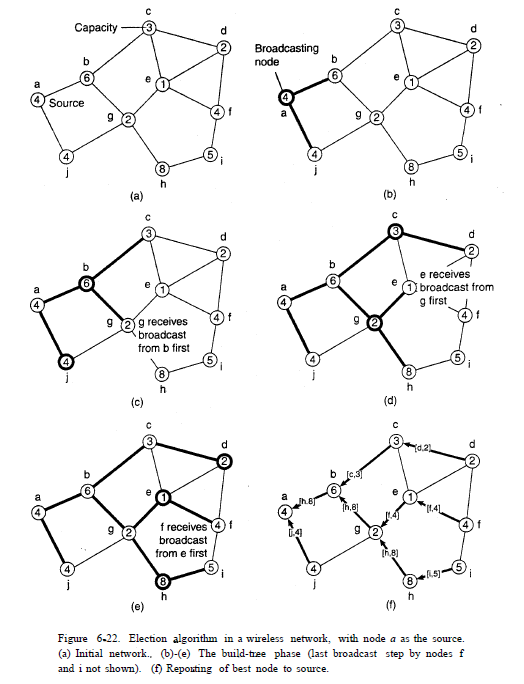
\includegraphics[width=400px]{gfx/Leader_adhoc.png}
	\caption{Election in wireless networks}
	\label{img:Leader_adhoc}
\end{figure}

\section{The Bully Algorithm(flooding) (Garcia-Mdina, 1982)}
- process P holds election
\begin{compactenum}
\item P sends ELECT message to all processes
\item P wins if there is no response $\Rightarrow$ P is leader and sends COORDINATOR message to all available nodes.
\item if Q answers with OK, Q takes over and sends ELECT again.
\end{compactenum}
\begin{figure}[h]
	\centering
	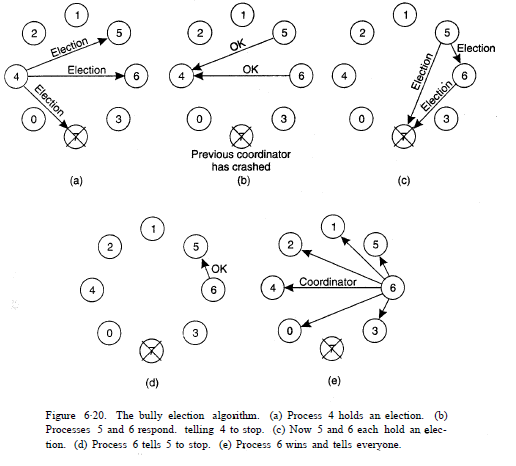
\includegraphics[width=400px]{gfx/leader1.png}
	\caption{The bully election algorithm}
	\label{img:leader1}
\end{figure}

%BILD DINGDINGDING

